\chapter{Grupos Cíclicos}
\label{cha:ciclicos}

No Capítulo \ref{cha:distribuicao-chaves} vimos que uma condição necessária para a segurança do protocolo de Diffie-Hellman é a dificuldade do problema do logaritmo discreto (DLog). 
Tanto o protocolo de Diffie-Hellman quanto o sistema de criptografia assimétrica de El Gammal assumem que podemos construir grupos cíclicos cujo problema DLog seja difícil.
Nesta seção apresentaremos duas construção de grupos cíclicos em que DLog é considerado difícil e ambas são usadas na prática.

\section{Grupos de ordem prima}
\label{sec:grupos-de-ordem}

O primeiro modelo parte de um teorema que estabelece que grupos com tamanho primo são necessariamente cíclicos e, além disso, qualquer elemento diferente da identidade é um gerador.

Vamos começar generalizando o Corolário \ref{cor:euler} do Teorema de Euler usado para provar a correção do algoritmo RSA.
Naquela situação estávamos usando um grupo específico, a saber, $\mathbb{Z}_n^\star$, mas o resultado vale para qualquer grupo finito: 


\begin{lemma}
   Seja $\mathbb{G}$ um grupo finito e $g \in \mathbb{G}$ um elemento de ordem $i$.
  Então para todo $x$ temos que $g^x = g^{[x\ mod\ i]}$.
\end{lemma}
\begin{proof}
Pelo algoritmo da divisão temos que $x = qi +r$ em que $r = [x\ mod\ i]$.
Portanto temos que:
\begin{displaymath}
  g^x = g^{qi + r} = g^{qi} \circ g^r = (g^i)^q \circ g^{[x\ mod\ i]} = g^{[x\ mod\ i]}
\end{displaymath}
\end{proof}

Agora podemos provar o seguinte teorema:

\begin{theorem}
  Se $\mathbb{G}$ é um grupo de ordem prima $p$ então $\mathbb{G}$ é cíclico e qualquer $g \in \mathbb{G}$ diferente de $1$ é um gerador.
\end{theorem}
\begin{proof}
  Seja $p = |\mathbb{G}|$ a ordem do grupo $\mathbb{G}$ e $i$ a ordem de um elemento qualquer $g \in \mathbb{G}$. 
  Pelo lema temos que $g^p = g^{[p\ mod\ i]}$ e pelo Teorema \ref{theo:gen-euler} temos que $g^p = 1$. 
  Como $[p\ mod\ i] < i$ e como, por definição, $i$ é o menor inteiro tal que $g^i = 1$ temos que $[p\ mod\ i] = 0$, ou seja, $i|p$.
  Mas, uma vez que $p$ é primo, temos que $i = 1$ ou $i = p$.
  O único elemento que tem ordem $1$ é a identidade, todos os demais tem ordem $p$ e, portanto, são geradores de $\mathbb{G}$.
\end{proof}

Esse resultado sugere que uma boa forma de encontrar grupos cíclicos é por buscando grupos de ordem prima.
Note, porém, que os candidatos naturais $\mathbb{Z}_p^\star$ tem ordem $p - 1$ o que quase nunca é primo\footnote{A única exceção é $p = 3$.}.
O que se costuma fazer é trabalhar com algum subgrupo de $\mathbb{Z}_p^\star$ de ordem prima.
O teorema a seguir, que não será provado, estabelece que se $p = qr + 1$ para algum $q$ primo, então o conjunto dos {\em $r$-ésimos resíduos módulo $p$}formam um grupo de tem tamanho $q$:

\begin{theorem}
Se $p = qr + 1$ e $p$ e $q$ são primos, então temos que
\begin{displaymath}
  \mathbb{G} = \{[h^r\ mod\ p] : h \in \mathbb{Z}_p\}
\end{displaymath}
é um subgrupo de $\mathbb{Z}_p^\star$ de ordem $q$.
\end{theorem}
   
Este teorema é o que garante a correção do seguinte algoritmo:

\begin{codebox}
\Procname{$\proc{GeradorDeGruposCiclicos}(1^n)$}
\li \Comment Recebe um parâmetro de segurança $1^n$ que estabelece $l = l(n)$
\li \Comment Devolve um grupo cíclico $\mathbb{G}$ cuja ordem é $q$ e um gerador $g$
\li escolhe aleatoriamente $q$ primo com $l$ bits
\li gera um primo $p$ tal que $q|(p-1)$
\li escolhe aleatoriamente $h \in \mathbb{Z}_p^\star$ tal que $h \neq 1$ 
\li $g \gets [h^{\frac{p-1}{q}}\ mod\ p]$
\li \Return $p, q, g$
\end{codebox}

O problema do logaritmo discreto para grupos gerados por esse algoritmo é considerado difícil.

\section{Curvas Elípticas}
\label{sec:curvas-elipticas}

Uma curva elíptica é formada por todos os pontos $(x,y)$ que satisfazem a seguinte equação, dados os parâmetro $a$ e $b$:

\begin{displaymath}
  y^2 = x^3 + ax + b 
\end{displaymath}

\begin{figure}[htbp]
  \centering
  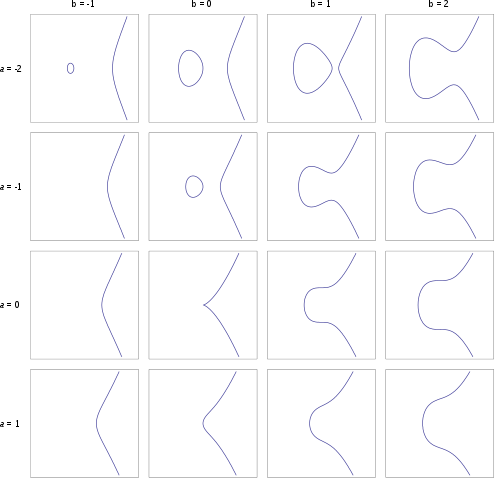
\includegraphics[width=.8\textwidth]{imagens/EllipticCurves.png}
  \caption{Curvas elípticas com diferentes parâmetros}
  \label{fig:curvas-elipticas}
\end{figure}

Podemos definir a adição de pontos em uma curva elíptica de maneira geometricamente natural.
A soma de dois pontos distintos é dada pelo ponto que intersecciona a reta que passa pelos dois (Figura \ref{fig:soma-eliptica} - quadro 1).
No caso extremo em que queremos somar o mesmo ponto duas vezes pegamos a reta tangente ao ponto e verificamos em qual ponto ela cruza com a reta (Figura \ref{fig:soma-eliptica} - quadro 2).
Nos casos degenerados em que a reta não cruza com a curva vamos atribuir um valor especial $0$ (Figura \ref{fig:soma-eliptica} - quadro 3).

\begin{figure}[htbp]
  \centering
  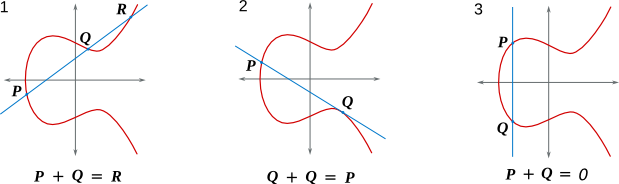
\includegraphics[width=\textwidth]{imagens/ECClines2.png}
  \caption{Soma de pontos em curvas elípticas}
  \label{fig:soma-eliptica}
\end{figure}

Algebricamente definimos a soma dos pontos da seguinte forma: $(x_1, y_1) + (x_2, y_2) = (x_3, y_3)$ tal que:

\begin{eqnarray*}
x_3 & = & s^2 - x_1 - x_2\\
y_3 & = & s(x_1 - x_3) - y_1  
\end{eqnarray*}

e $s$ (a inclinação da reta) na apresentação geométrica é dada por:

\begin{displaymath}
  s =\left\{
  \begin{array}{cl}
    \frac{y_2 - y_1}{x_2 - x_1} & \textrm{se os pontos são distintos}\\
    \frac{3x_1^2 + a}{2y_1} & \textrm{caso contrário}\\
  \end{array}\right .
\end{displaymath}


O conjunto $(\mathbb{R} \times \mathbb{R}) \cup \{0\}$ junto da operação que acabamos de definir é um grupo, porém, infinito.

Para nos mantermos no mundo dos grupos finitos estabeleceremos um número primo $p$ e faremos todas as contas acima módulo $p$ -- o que faz com que não sejamos mais capazes de expressar nossas contas de maneira geometricamente intuitiva.

Vamos então escrever o conjunto dos elementos de uma curva elíptica como:
\begin{displaymath}
  E(\mathbb{Z}_p) = \{(x,y) : x, y \in \mathbb{Z}_p \textrm{ e } y^2 \equiv x^3 + ax + b\ mod\ p\} \cup \{0\}
\end{displaymath}

O teorema a seguir nos dá algumas pistas sobre o tamanho deste conjunto:


\begin{theorem}[Hasse]
  Seja $p$ um número primo, então temos que:
\begin{displaymath}
  p + 1 - 2\sqrt{p} \leq |E(\mathbb{Z}_p)| \leq p + 1 + 2\sqrt{p} 
\end{displaymath}
\end{theorem}

Ou seja, o número de pontos em $E(\mathbb{Z}_p)$ é mais ou menos da mesma ordem do que $p$.
Podemos então construir o seguinte algoritmo análogo ao apresentado na seção anterior para computar um grupo cíclico:


\begin{codebox}
\Procname{$\proc{GeradorDeGruposCiclicos2}(1^n)$}
\li \Comment Recebe um parâmetro de segurança $1^n$
\li \Comment Devolve um grupo cíclico $\mathbb{G}$ cuja ordem é $q$ e um gerador $g$
\li escolhe aleatoriamente $p$ primo com $n$ bits
\li \While $q$ não for primo 
\li \Do escolha $a, b$ aleatoriamente em $\mathbb{Z}_p$ tal que $4a^3 + 27b^2 \neq 0\ mod\ p$
\li defina a curva elíptica $E(\mathbb{Z}_p)$
\li seja $q = |E(\mathbb{Z}_p)|$
\End
\li escolha um elemento qualquer $g \in E(\mathbb{Z}_p) \setminus \{0\}$
\li \Return $(a, b, p), q, g$
\end{codebox}

O logaritmo discreto de um grupo tal qual construído pelo algoritmo acima é considerado difícil.